\documentclass[11pt]{article}
\usepackage{verbatim}
\usepackage{listings}
\usepackage{graphicx}
\usepackage{a4wide}
\usepackage{color}
\usepackage{amsmath}
\usepackage{amssymb}
\usepackage[dvips]{epsfig}
\usepackage[T1]{fontenc}
\usepackage{cite} % [2,3,4] --> [2--4]
\usepackage{shadow}
\usepackage{hyperref}
\usepackage{physics}
\usepackage{url}
\usepackage{tikz}
\usepackage{subcaption}
\usepackage[utf8]{inputenc}
\usepackage{booktabs} % Allows the use of \toprule, \midrule and \bottomrule in tables





\usetikzlibrary{arrows, shapes}

\setcounter{tocdepth}{2}

\lstset{language=c++}
\lstset{alsolanguage=[90]Fortran}
\lstset{basicstyle=\small}
\lstset{backgroundcolor=\color{white}}
\lstset{frame=single}
\lstset{stringstyle=\ttfamily}
\lstset{keywordstyle=\color{red}\bfseries}
\lstset{commentstyle=\itshape\color{blue}}
\lstset{showspaces=false}
\lstset{showstringspaces=false}
\lstset{showtabs=false}
\lstset{breaklines}

\title{ Computational Physics II \\ FYS-4411 }
\author{Gullik Vetvik Killie\\
		Håkon S.B. Mørk\\
		Jose Emilio Ruiz Navarro
		}

\begin{document}

\maketitle

\abstract{In this work, a simple Variational Monte Carlo (VMC) method has been used to calculate the values of the energies of the ground states of two atoms: helium and beryllium. In the case of helium, the average distance between the electrons was computed as well, and two different hydrogen-like wavefunctions were used: one without taking into account the interaction between the two electrons and another one with a Jastrow factor dependent on the distance between the electrons $r_{12}$. The dependence on the timestep of the algorithm and the results was investigated as well, and no significant relation was found. Importance sampling was introduced as well to improve the program with more efficiency and make the results more precise. We provide a statistical analysis by the means of blocking so as to not understimate the error of our results. The one-body and charge densities were obtained to compare the effects of the Jastrow factor with and provide insight into the electronic structure of the beryllium atom.}

\section{Introduction}

VMC methods pose a very attractive alternative to other more complex ways of finding the ground state energies of simple atoms and molecules, like configuration-interaction calculations. The price to be paid in exchange for this simplicity is the sensitivity to the trial wave functions that are used, a VMC algorithm is very sensitive to how these are constructed, so they are one of the most important aspects to be considered (in this work, given the simple nature of the atoms which we will be working with, it's not so important to worry about the quality of the trial wave functions because very simple and basic ones are more than enough to reproduce the actual results). It shouldn't be forgotten that it is a variational method, and this implies that finding the optimal set of variational parameters is going to be the most important part of the calculation itself because it create a lot of problems if the search range for the parameters is illy defined and is not close enough to the variational minimum, namely, the results will have a poor quality if this happens. This means that the parameters need to be chosen very carefully, or a recursive search with decreasingly coarse spacing in the space of variational parameters is required if there is no deep knowledge about the system in question.\\

Instead of evaluating a very complex multidimensional integral to compute the expectation value of an operator, like the hamiltonian in this case, a VMC calculation exploits the fact that the majority of the configuration space where the wave function belongs can be regarded as much less important than other parts, the values of the wave function are too small there and can be mostly ignored during the integration of the algorithm. To capitalize this, the Metropolis algorithm is added to the VMC method, as well as importance sampling.\\


\section{Methods}
	\subsection{Monte Carlo of the Helium Atom}
		In a quantum mechanical system the energy is given by the expectation value of the Hamiltonian, let \(\Psi_T\) be a proposal for a wavefunction that can describe the system.

		\begin{align}
			E[\hat{H}] = \expval{\hat{H}}{\Psi_T} = \frac{\int{d\vb{R} \Psi_T^*(\vb{R})\hat{H} \Psi_T(\vb{R})  }}{ \int{d\vb{R} \Psi_T^*(\vb{R}) \Psi_T(\vb{R}) }}
		\end{align}

		Let us introduce a local energy: 

		\begin{align}
			E_L(\hat{H}) &= \frac{1}{ \Psi_T(\vb{R}) } \hat{H} \Psi_T(\vb{R}))
		\end{align}

		\begin{align}
			E[\hat{H}] &= \frac{\int{d\vb{R} \Psi_T^*(\vb{R}) \Psi_T(\vb{R}) E_L(\vb{R}))  }}{ \int{d\vb{R} \Psi_T^*(\vb{R}) \Psi_T(\vb{R}) }}
			\intertext{Since the denumeraor is a scalar constant after integrating it we can put it inside the integral in the numerator}
			E[\hat{H}] &= \int{d\vb{R} \frac{\Psi_T^*(\vb{R}) \Psi_T(\vb{R})  }{\int{d\vb{R'} \Psi_T^*(\vb{R'}) \Psi_T(\vb{R'})}}  E_L(\vb{R})  }
			\\
			E[\hat{H}] &= \int{d\vb{R} P(\vb{R}) E_L(\vb{R}) }
		\end{align}

			This probability function with \(P(\vb{R})\) as the pdf, and we can use monte carlo integration to solve the integral. 

		\begin{enumerate}
			\item Initialise system. Give particles a random position and decide how many Monte Carlo Cycles to run.
			\item Start Monte Carlo Calculations
				\begin{enumerate}
					\item Propose a move of the particles according to an algorithm, for example \newline \( \vb{R_{new}} = \vb{R_{old}} + \delta * r \), where \(r\) is a random number in \([0,1]\)
					\item Accept or reject move according to \( P(\vb{R_{new}})/ P(\vb{R_{old}}) \ge r \), where r is a new number. Update position values if accepted.
					\item Calculate energy for this cycle.
				\end{enumerate}
		\end{enumerate}

	\subsection{Helium atom}
		The dimensionless hamiltonian for the Helium atom consists of a kinetic energy part and a potential energy part and is given by

		\begin{align}
			\hat{H} &= -\frac{\nabla^2_1}{2} - \frac{\nabla^2_2}{2} - \frac{Z}{r_1} - \frac{Z}{r_2} + \frac{1}{r_{12}}
		\end{align}

		For the energy to be finite the wavefunction must be constructed so the local energy is finite at all points.

		\begin{align}
			E_L(r_i,r_{12}) &= \frac{1}{\Psi_T} \hat{H} \Psi_T
		\end{align}

		If we consider the case where \(r_i \rightarrow 0\) then the \(- \frac{\nabla^2_i}{2} - \frac{Z}{r_i} \) terms of the hamiltonian could cause the energy to blow up, so we need to make sure that those terms stay finite in the limit.

		\begin{align}
			\lim_{r_i\rightarrow 0} {E_L(r_1,r_{12}) } &= \frac{1}{R_i(r_i)} \left( - \frac{1}{2}\pdv[2]{}{x_k} - \frac{Z}{r_i} \right) R_i(r_i) + G(r_i, r_{ij})
			\\
			\lim_{r_i\rightarrow 0} {E_L(r_1,r_{12}) } &= \frac{1}{R_i(r_i)} \left( - \frac{1}{2}\pdv[2]{}{r_k} - \frac{1}{r_i}\pdv{}{r_i}	 -	 \frac{Z}{r_i} \right) R_i(r_i) + G(r_i, r_{ij})
			\intertext{ Derivatives of the wavefunction does not diverge since the wavefunction is finite at all points. so the following terms dominate when the particles approach the center. }
			\lim_{r_i\rightarrow 0} {E_L(r_1,r_{12}) } &= \frac{1}{R_i(r_i)} \left( - \frac{1}{r_i}\pdv{}{r_i}	 -	 \frac{Z}{r_i} \right) R_i(r_i)
			\end{align}

		\begin{align}
			 \frac{1}{R_i(r_i)} \pdv{}{r_i} R_i(r_i)	=  -Z  \qquad{ \text{ With solution }}  \qquad R_i(r_i) = A e^{-Z}
		\end{align}

		A similar calculation applies for \(r_{12} \rightarrow 0\) and a trialfunction of the form   \[\Psi_T(r_1,r_2,r_{12}) = e^{-\alpha (r_1 + r_2)} e^{\beta r_{12}} \] should fulfill the condition that the wavefunction is finite everywhere.


	\subsection{Beryllium atom}

		It is fairly simple to extend the calculational machinery of Variational
		Monte Carlo to other systems than the Helium atom. To show this we
		want to perform calculations on the beryllium atom. As beryllium has
		four electrons compared to the 2 of helium, we need to calculate a
		Slater determinant. However the computation of the Slater determinant
		can be simplified for beryllium. Sticking to hydrogen-like wave functions,
		we can write the trial wave function for beryllium as
		\begin{equation}
			\psi_{T}({\bf r_{1}},{\bf r_{2}},{\bf r_{3}},{\bf r_{4}})=Det\left(\phi_{1}({\bf r_{1}}),\phi_{2}({\bf r_{2}}),\phi_{3}({\bf r_{3}}),\phi_{4}({\bf r_{4}})\right)\prod_{i<j}^{4}\exp{\left(\frac{r_{ij}}{2(1+\beta r_{ij})}\right)},
		\end{equation}
		where $Det$ is a Slater determinant and the single-particle wave
		functions are the hydrogen wave functions for the 1s and 2s orbitals.
		With the variational ansatz these are
		\[
		\phi_{1s}({\bf r_{i}})=e^{-\alpha r_{i}},
		\]
		and 
		\[
		\phi_{2s}({\bf r_{i}})=\left(1-\alpha r_{i}/2\right)e^{-\alpha r_{i}/2}.
		\]
		The Slater determinant for the ground state of the Beryllium atom
		can be approximated as
		\[
		\psi_{T}({\bf r_{1}},{\bf r_{2}},{\bf r_{3}},{\bf r_{4}})\propto\left(\phi_{1s}({\bf r_{1}})\phi_{2s}({\bf r_{2}})-\phi_{1s}({\bf r_{2}})\phi_{2s}({\bf r_{1}})\right)\left(\phi_{1s}({\bf r_{3}})\phi_{2s}({\bf r_{4}})-\phi_{1s}({\bf r_{4}})\phi_{2s}({\bf r_{3}})\right).
		\]


		Furthermore, for the Jastrow factor, 
		\[
		\Psi_{C}=\prod_{i<j}g(r_{ij})=\exp{\left\{ \sum_{i<j}\frac{ar_{ij}}{1+\beta r_{ij}}\right\} },
		\]
		we need to take into account the spins of the electrons. We fix electrons
		1 and 2 to have spin up, and electron 3 and 4 to have spin down. This
		means that when the electrons have equal spins, we get
		\[
		a=\frac{1}{4},
		\]
		and if they have opposite spins, we get
		\[
		a=\frac{1}{2}.
		\]

	


	\subsection{Derivation of local energies}
		The local energy of is dependant on the Hamiltonian and the wavefunction describing the system, the Hamiltonian incorporates both a kinetic energy part given by \( \frac{\nabla_i^2}{2} \) for each particle
		and a potential energy part given by \(\frac{Z}{r_i}\) and \(\frac{1}{r_{ij}}\), where \(Z\) is the charge of the center, \(r_i\) is the distance for electron \(i\) to the atom center and \(r_{ij}\) is the distance between electron \(l\) and \(m\). Then the local energy is given by the following:

		\begin{align}
			E_L &= \sum_{i,i<j}{\frac{1}{ \Psi_T(\vb{r_i} , \vb{r_{ij}}) } \hat{H} \Psi_T(\vb{r_i} , \vb{r_{ij}})}
			\\
			&=	\sum_{i,i<j}\frac{1}{ \Psi_T(\vb{r_i} , \vb{r_{ij}}) } \left( - \frac{\nabla_i^2}{2} -\frac{Z}{r_i}  -  \frac{Z}{r_j} +  \frac{1}{r_{ij} }  \right) \Psi_T(\vb{r_i} , \vb{r_{ij}})
			\\
			&= \sum_{i,i<j}{-\frac{1}{2\Psi_T} \left(\nabla_i^2 \Psi_T  \right)  -\frac{Z}{r_i}  -  \frac{Z}{r_j} +  \frac{1}{r_{ij} }}
		\end{align}

		Let us change derivation variables:

		\begin{align}
			-\frac{1}{2\Psi_T} \left(\nabla_i^2 \Psi_T  \right) &= \sum_{m=1}^{3}{-\frac{1}{2\Psi_T} \left( \pdv[2]{\Psi_T}{x_m} \right)_i}
			\\
			&= \sum_{m=1}^{3}{-\frac{1}{2\Psi_T} \left( \pdv{}{x_m} \left( \pdv{\Psi_T}{r_i}\pdv{r_i}{x_m} \right) \right)_i}
			\intertext{Since \(r_i = \left( x_1^2 + x_2^2 + x_3^2 \right)^{1/2}\) then \( \pdv{r_i}{x_m} = \pdv{\left( x_1^2 + x_2^2 + x_3^2 \right)^{1/2}}{x_m} =\frac{x_m}{r_i} \)}
			&= \sum_{m=1}^{3}{-\frac{1}{2\Psi_T} \left( \pdv{}{x_m} \left( \pdv{\Psi_T}{r_i}\frac{x_m}{r_i} \right) \right)_i}
			\\
			&= \sum_{m=1}^{3}{-\frac{1}{2\Psi_T} \left( \pdv{\Psi_T}{x_m}{r_i}\frac{x_m}{r_i} + \pdv{\Psi_T}{r_i} \pdv{}{x_m} \left(\frac{x_m}{r_i} \right) \right)_i}
			\intertext{ The term \( \pdv{}{x_m} \left(\frac{x_m}{r_i} \right) \) becomes for the different values for \(m\),  \(\pdv{}{x_1}  \left( \frac{x_1}{\left( x_1^2 + x_2^2 + x_3^2 \right)^{1/2}} \right) = \frac{x_2^2 + x_3^2}{r_i^3}\) so all the values for \(m\) term it should sum up to \( \frac{ 2 (x_1^2 + x_2^2 + x_3^2) }{ r_i^3 } \) }
			&= -\frac{1}{2\Psi_T} \left( \pdv[2]{\Psi_T}{r_i}\frac{x_1^2 + x_2^2 + x_3^2}{r^2_i} + \pdv{\Psi_T}{r_i} \frac{ 2 (x_1^2 + x_2^2 + x_3^2) }{ r_i^3 } \right)_i
			\\
			&= -\frac{1}{2\Psi_T} \left( \pdv[2]{\Psi_T}{r_i} + \pdv{\Psi_T}{r_i} \frac{ 2 }{ r_i } \right)
		\end{align}
		Then the local energy becomes:
		\begin{align}
			E_L = \sum_{i,i<j}{  -\frac{1}{2\Psi_T} \left( \pdv[2]{\Psi_T}{r_i} + \pdv{\Psi_T}{r_i} \frac{ 2 }{ r_i } \right)  -\frac{Z}{r_i}  -  \frac{Z}{r_j} +  \frac{1}{r_{ij} }} \label{eq:localEnergy}
		\end{align}


		\subsubsection{Helium: Simple trialfunction}
		The simple version of the trial function is only dependant on one parameter \( \alpha \) and does not take into account interaction between the two electrons, it is of the form 
		\[ \Psi_T (\vb{r_1}, \vb{r_2}) = \exp{ -\alpha (r_1 + r_2) } \]Let us set this trialfunction into the equation for the local energy \eqref{eq:localEnergy}.
		\begin{align}
			E_L &= \sum_{i,i<j}{  -\frac{1}{2\Psi_T} \left( \pdv[2]{e^{-\alpha (r_i + r_j)}}{r_i} + \pdv{e^{-\alpha (r_i + r_j)}}{r_i} \frac{ 2 }{ r_i } \right)  -\frac{Z}{r_i}  -  \frac{Z}{r_j} +  \frac{1}{r_{ij} }} 
			\\
			E_L &= -\frac{1}{2\Psi_T} \sum_{i=1}^2{ \left( \alpha^2 -\alpha \frac{ 2 }{ r_i } \right) \Psi_T  -\frac{Z}{r_i} +  \frac{1}{r_{ij} } }
			\\
			E_L &= -\alpha^2 + (\alpha-Z) \left( \frac{1}{r_1} + \frac{1}{r_2} \right) + \frac{1}{r_{12}} 
		\end{align}



\subsection{Importance sampling}

We now want to make the code more efficient, so we replace the brute
force Metropolis algorithm with a walk in coordinate space biased
by the trial wave function, an approach based on the Fokker-Planck
equation and the Langevin equation for generating a trajectory in
coordinate space. 

For one particle or walker, a diffusion process characterized by a
time-dependent probability density $P\left(x,t\right)$ in one dimension
we have the Fokker-Planck equation
\[
\frac{\partial P}{\partial t}=D\frac{\partial}{\partial x}\left(\frac{\partial}{\partial x}-F\right)P\left(x,t\right),
\]
where $F$ is a drift term and $D$ is the diffusion coefficient. 

The new positions in coordinate space are found using the Langevin
equation with Euler's method. We go from the Langevin equation
\[
\frac{\partial x(t)}{\partial t}=DF(x(t))+\eta
\]
where$\eta$ is a random variable. This gives us a new position
\[
y=x+DF(x)\Delta t+\xi\sqrt{\Delta t}.
\]
Here $\xi$ is gaussian random variable and $\Delta t$ is a chosen
time step. $D$ comes from the factor $1/2$ in the kinetic energy
operator, and is therefore equal to $1/2$ in atomic units.

The process of isotropic diffusion characterized by a time-dependent
probability density $P\left(\mathbf{x},t\right)$ will, as an approximation,
obey the Fokker-Planck equation
\[
\frac{\partial P}{\partial t}=\sum_{i}D\frac{\partial}{\partial\mathbf{x_{i}}}\left(\frac{\partial}{\partial\mathbf{x_{i}}}-\mathbf{F_{i}}\right)P(\mathbf{x},t),
\]
where $\mathbf{F}_{i}$ is component number $i$ of the drift term
caused by an external potential, and $D$ is the diffusion coefficient.
We set the left hand side equal to zero and obtain the convergence
to a stationary probability density
\[
\frac{\partial^{2}P}{\partial{\mathbf{x_{i}}^{2}}}=P\frac{\partial}{\partial{\mathbf{x_{i}}}}\mathbf{F_{i}}+\mathbf{F_{i}}\frac{\partial}{\partial{\mathbf{x_{i}}}}P.
\]


Inserting the drift vector, $\mathbf{F}=g(\mathbf{x})\frac{\partial P}{\partial\mathbf{x}}$,
we get
\[
\frac{\partial^{2}P}{\partial{\mathbf{x_{i}}^{2}}}=P\frac{\partial g}{\partial P}\left(\frac{\partial P}{\partial{\mathbf{x}_{i}}}\right)^{2}+Pg\frac{\partial^{2}P}{\partial{\mathbf{x}_{i}^{2}}}+g\left(\frac{\partial P}{\partial{\mathbf{x}_{i}}}\right)^{2}
\]
To meet the condition of stationary density the left hand side has
to be zero. This means that the terms containing first and second
order derivatives has to cancel each other, which is only possible
if $g=\frac{1}{P}$. This yields
\[
\mathbf{F}=2\frac{1}{\Psi_{T}}\nabla\Psi_{T},
\]
known as the quantum force. This so-called force pushes the walker
towards regions of configuration space where the trial wave function
is large, thus increasing the efficiency of the simulation. This is
a great improvement on the Metropolis algorithm where the walker has
the same probability to move in every direction.

From the Fokker-Planck equation we get a transition probability given
by Green's function
\[
G(y,x,\Delta t)=\frac{1}{(4\pi D\Delta t)^{3N/2}}\exp{\left(-(y-x-D\Delta tF(x))^{2}/4D\Delta t\right)}
\]
This means that the Metropolis algorithm
\[
A(y,x)=\mathrm{min}(1,q(y,x))),
\]
where 
\[
q(y,x)=\frac{|\Psi_{T}(y)|^{2}}{|\Psi_{T}(x)|^{2}},
\]
is replaced by the Metropolis-Hastings algorithm,
\[
q(y,x)=\frac{G(x,y,\Delta t)|\Psi_{T}(y)|^{2}}{G(y,x,\Delta t)|\Psi_{T}(x)|^{2}}
\]


		\subsection{Blocking}
			Blocking refers to a method to more accurately estimate the error of the values obtained by the VMC algorithm. It's actually a completely separate and independent process. The basic idea lies on the correlations between all the measurements. If these are important enough, they will produce an increase in the error that needs to be taken into account. The reason behind this is related to the effective amount of measurements, if there are correlations there will be measurements that will contain less information, so these won't be as valuable as the rest and it will be as if there are \textit{less} measurementes than we actually have. Obviously this is a problem, the usual identification of the error with $\sqrt{\frac{\sigma}{n}}$ will be overly optimistic and a correction is needed.\\

\[
f_d=\frac{1}{n-d}\sum_{k=1}^{n-d}{\left(x_k-\bar{x}_n\right)\left(x_{k+d}-\bar{x}_n\right)}
\]


			The solution is to use blocking, and the algorithm to do this is actually quite simple. The total amount of measurements is divided into blocks (hence the name) of a certain size, and for each block the standard deviation is obtained. When the standard deviation stops increasing as the block size does, the correlations are irrelevant and the value for it is set


			\begin{figure}
\centering 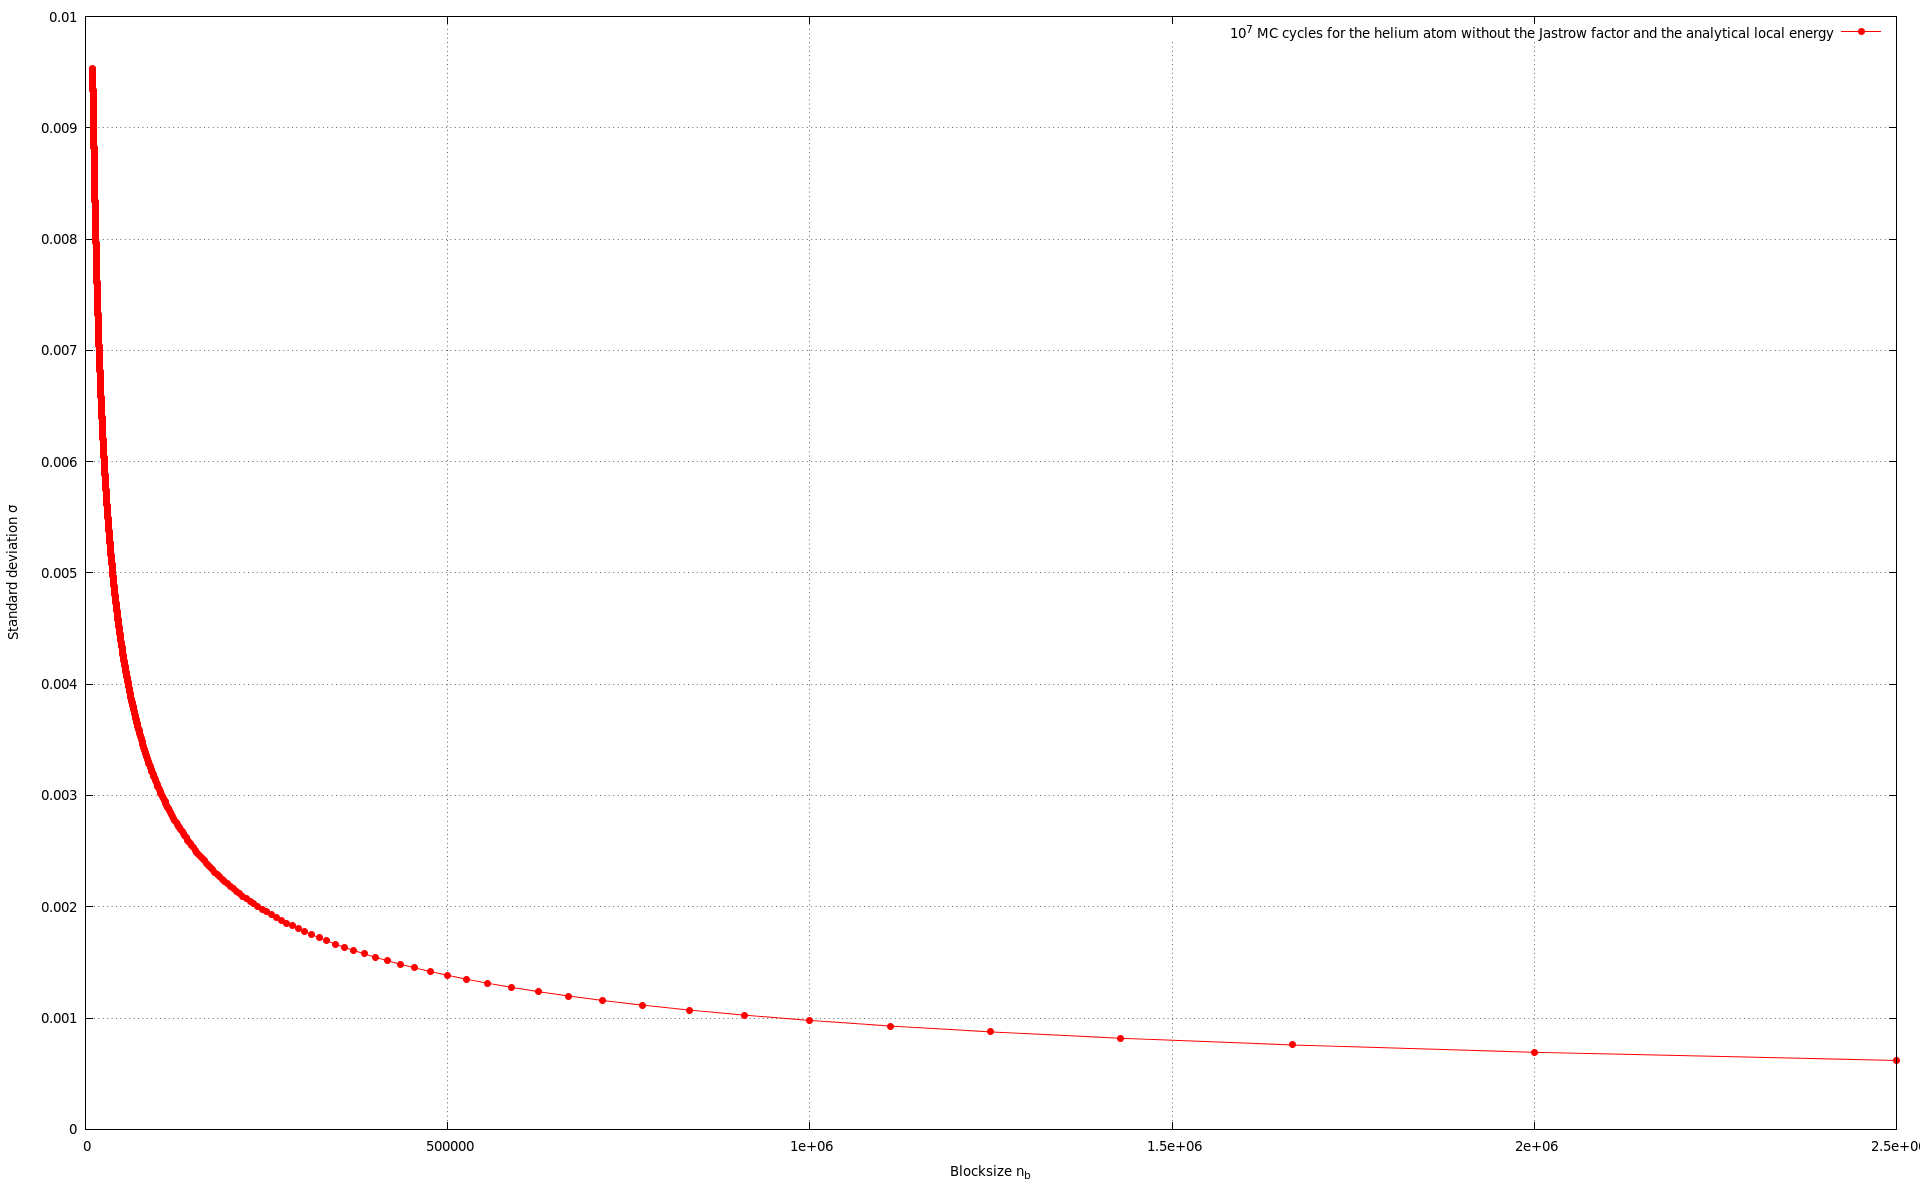
\includegraphics[width=0.45\linewidth]{figures/blockingheliumsimpleandalytical}
\protect\caption{STD vs. blocksize. Here we see the trend }
\label{fig01:alpha_Simple} 
\end{figure}



\section{Results and discussion}
	

As a first attempt to solve the ground state energy for the helium
atom we perform Variational Monte Carlo calculation with a brute force
Metropolis sampling. We do this with two trial wave functions
\[
\psi_{T1}({\bf r_{1}},{\bf r_{2}},{\bf r_{12}})=\exp{\left(-\alpha(r_{1}+r_{2})\right)}
\]
and 
\[
\psi_{T2}({\bf r_{1}},{\bf r_{2}},{\bf r_{12}})=\exp{\left(-\alpha(r_{1}+r_{2})\right)}\exp{\left(\frac{r_{12}}{2(1+\beta r_{12})}\right)},
\]
using $\alpha$ and $\beta$ as variational parameters. Energy values
for the simple wave function, $\psi_{T1}$, using only one variational
parameter $\alpha$, are shown in figure \ref{fig01:alpha_Simple}.
We run the Variational Monte Carlo calculation with $10^{7}$ cycles.
As we see in the figures, the energy minimum occurs when we use $\alpha=1.65$.
Using this value for $\alpha$ we get an energy of $-2.8442934$. 
The parameter $\alpha$ can be interpreted as a parameter for the
force pulling the electron to the nucleus. 

\begin{figure}
\centering 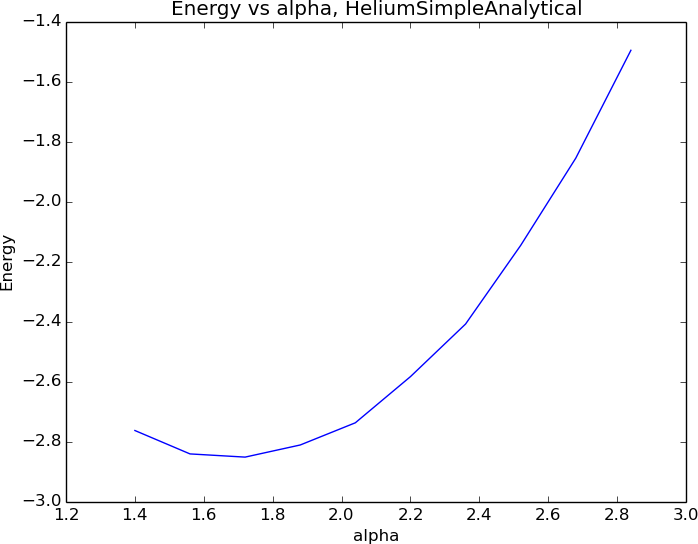
\includegraphics[width=0.45\linewidth]{figures/EnergyVsAlphaHeliumSimpleAnalytical}
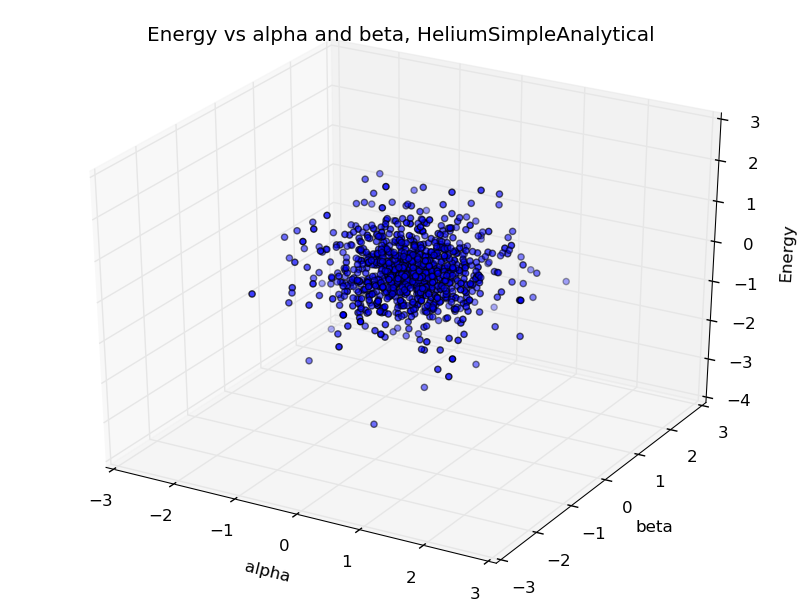
\includegraphics[width=0.45\linewidth]{figures/VarianceVsAlphaHeliumSimpleAnalytical}
\protect\caption{To be filled in}
\label{fig01:alpha_Simple} 
\end{figure}


\begin{figure}
\centering 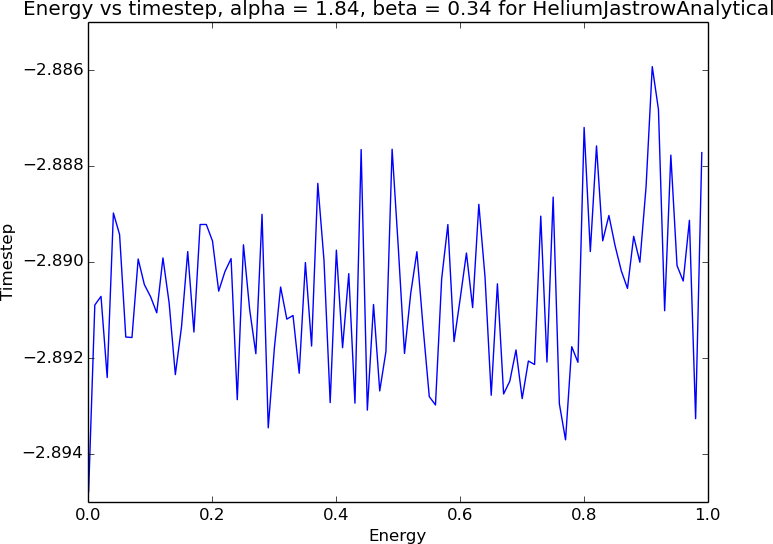
\includegraphics[width=0.45\linewidth]{figures/HeliumJastrowAnalyticalTimeEnergy}
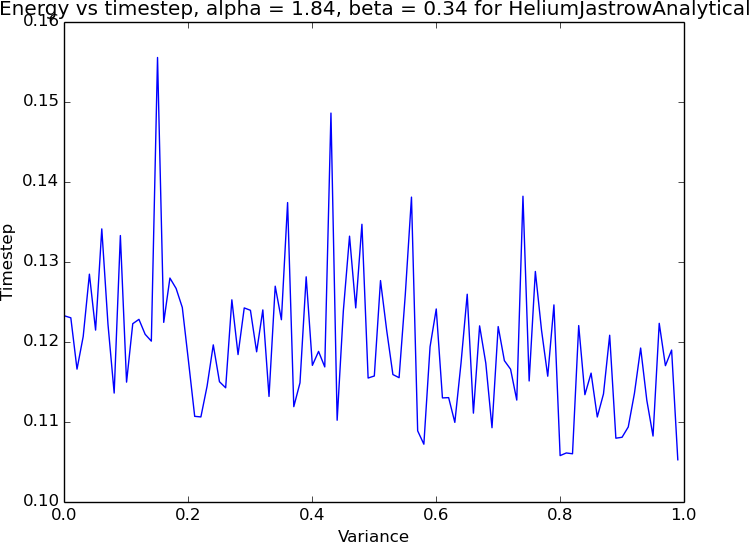
\includegraphics[width=0.45\linewidth]{figures/HeliumJastrowAnalyticalTimeVariance}
\protect\caption{To be filled in}
\label{fig02:timestep} 
\end{figure}

We now look at our second trial function, $\psi_{T2}$. Running over
different values for the two variables $\alpha$ and $\beta$, again
with $10^{7}$ cycles in the Monte Carlo simulation, we get the results
presented in figure \ref{fig03:AlphaBeta}. From this run we find
that the optimal values are $\alpha=1.8$ and $\beta=0.94$, and we
get a minimum energy of $-2.8979105$, which is considerably better
than without the Jastrow factor.

\begin{figure}
\centering 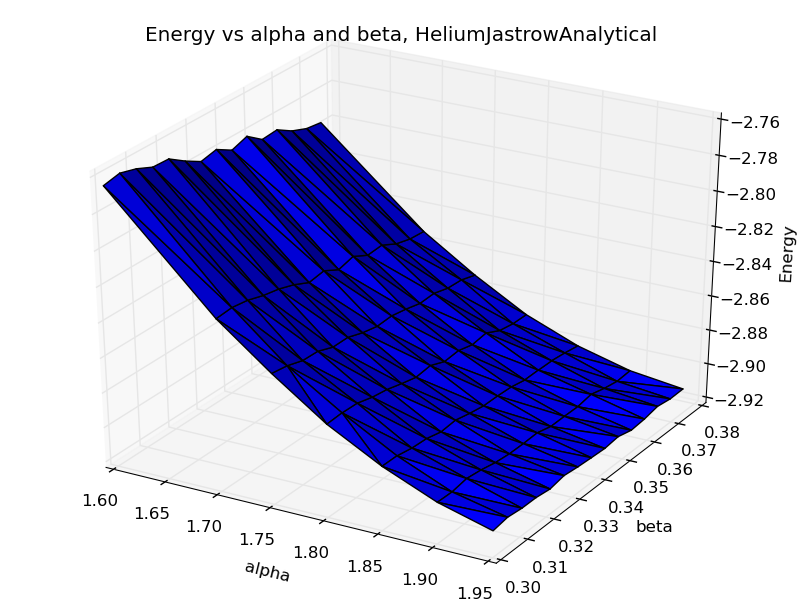
\includegraphics[width=0.45\linewidth]{figures/HeliumJastrowAnalyticalAlphaBetaEnergy}
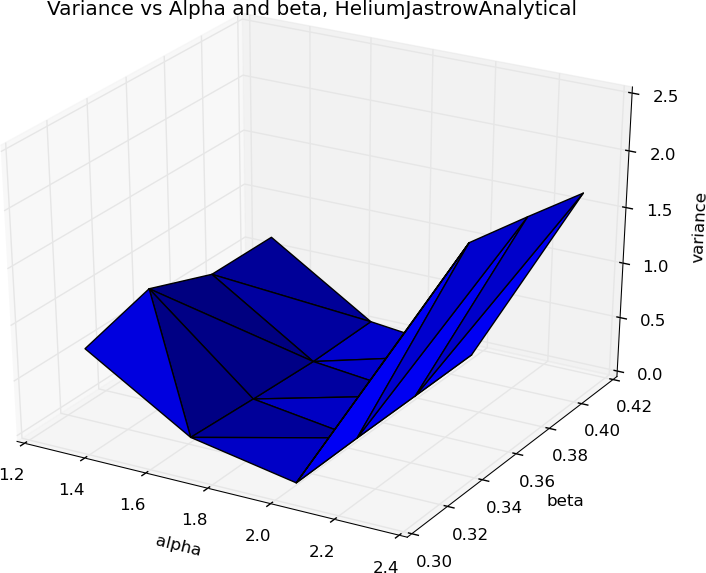
\includegraphics[width=0.45\linewidth]{figures/HeliumJastrowAnalyticalAlphaBetaVariance}
\protect\caption{To be filled in}
\label{fig03:AlphaBeta} 
\end{figure}

Finally we use our Variational Monte Carlo machinery to find the ground
state energy for a beryllium atom. Since beryllium has 4 electrons,
compared to the 2 in helium, the computation is much slower and we
only had time to run it for $10^{6}$ cycles. We then find the lowest
energy to be $-14.4127$ with $\alpha=3.8$ and $\beta=0.293$. 

From reseach papers we find the value for energy in the ground state
of helium to be $-2.9037$ {[}Toichiro Kinoshita{]} and the value
for energy in the ground state of beryllium to be $-14.667$ {[}Jacek
Koput{]}. In table \ref{EnergyComparisonTable} we compare results
obtained with our Variational Monte Carlo method with results from
various research papers. 

\begin{table}
\centering %
\begin{tabular}{|c|c|c|}
\hline 
Atom & VMC & References\tabularnewline
\hline 
\hline 
Helium $\psi_{T1}$ & $-2.8442$ & $-2.9037$ \tabularnewline
\hline 
Helium $\psi_{T2}$ & $-2.8979$ & $-2.9037$ \tabularnewline
\hline 
Beryllium & $-14.4127$ & $-14.667$\tabularnewline
\hline 
\end{tabular}

\protect\caption{Comparison of energies found with Variational Monte Carlo method and
energies found in research papers.}


\end{table}

\subsection{Alpha and Beta Values}

\begin{table}
\center
		\begin{tabular}{| c | c| c |}
		    \hline
		   	\textbf{Trialfunction} & \(\mathbf{\alpha}\) & \(\mathbf{\beta}\)
		    \\ \hline
		    Helium $\psi_{T1}$ & 1.65 & -
		    \\ \hline 
		    Helium $\psi_{T2}$ & 1.8 & 0.94
		    \\	\hline 
		    Beryllium $\psi_{T2}$	& 3.8	&	 0.293
		    \\ \hline
	  \end{tabular}
	  \caption{The values for \(\alpha\) and \( \beta \) where found by doing running Monte Carlo calculation with over a mesh of different \(\alpha\) and \( \beta \) values, with stepssize \(0.02\). Each Monte Carlo run went over \(10 000 000\), using importance sampling. Then the run with the lowest energy gave the \(\alpha\) and \(\beta\) values}
	  \label{tab:alpha_beta}
\end{table}

	Table \ref{tab:alpha_beta} shows the values, for \(\alpha\) and \(\beta\) values, we got from  running several Monte Carlo cycles with different values. As an algorithm to pick out the best values we minimized the energy found in the Monte Carlo runs. The values found are quite uncertain since the variance of the energy was quite high compared to the difference caused by varying the parameters. The variance was more smooth as a function of the parameters, see fig \ref{fig03:AlphaBeta} and should have been used.


	\subsection{Computational speed gain by using an analytical local energy}
	By using an analytical expression for the local energy instead of using a numerical derivation in the calculation a speed up of approximately factor \(4\) was achieved, see table \ref{tab:analyticVSNumeric}. 


	\begin{table}
\center
		\begin{tabular}{| c | c | c | c |}
		    \hline
		   	\textbf{Trialfunction} & Numerical (s) & Analytical (s) & Ratio
		    \\ \hline
		    Helium $\psi_{T1}$ & 61.75 & 14.34 & 4.307
		    \\ \hline 
		    Helium $\psi_{T2}$ & 86.76 & 19.98	& 4.342
		    \\	\hline 
		    Beryllium $\psi_{T2}$  	& &	 &
 		    \\ \hline
	  \end{tabular}
	  \caption{The time to run a Monte Carlo run with \(10^7\) cycles. The closed expression for the local energy increased the computation time by a significant degree for each trialfunction }
	  \label{tab:analyticVSNumeric}
\end{table}

\section{Conclusions and perspectives}

	\subsection{Parameter grid  and values }
		The algorithm by just minimizing the energy to find the best fits for \(\alpha\) and \(\beta\) could be improved since both the energy and it's variance should be minimized with a correct wavefunction. So the algorithm should take into account that and find the combined lowest energy and variance and use that to find the best values for the parameters. A homogeneous is used to search through the different \(\alpha\) and \(\beta\) and by improving this the speed of the program would be greatly improved. If for example it first did a coarse run, then found the best value searched in the vicinity of that point with a higher resolution it would be improved.


\appendix
	
	\section{Testing the VMC}
		\subsection{Hydrogen Atom}
			The wavefunction for the Helium atom can be found exactly and can be used to test our Variational Monte Carlo Calculation since an exact wavefunction should return the exact energy, \( 0.5 \) atomic units with \(0\) variance.

			\[ \Psi(\vb{R}) = r_1 e^{-r_1}  \qquad E_L(r_1) = -\frac{1}{r_1} - \frac{\alpha}{2} \left( \alpha - \frac{2}{r_1} \right) \]

			The unit test a unit named Helium tests the VMC clalculation with a hydrogen wavefunction and returns the correct values.



\end{document}


